\RequirePackage[l2tabu, orthodox]{nag}
\documentclass[version=3.21, pagesize, twoside=off, bibliography=totoc, DIV=calc, fontsize=12pt, a4paper]{scrartcl}
%Permits to copy eg x ⪰ y ⇔ v(x) ≥ v(y) from PDF to unicode data, and to search. From pdfTeX users manual. See https://tex.stackexchange.com/posts/comments/1203887.
	\input glyphtounicode
	\pdfgentounicode=1
%Latin Modern has more glyphs than Computer Modern, such as diacritical characters. fntguide commands to load the font before fontenc, to prevent default loading of cmr.
	\usepackage{natbib}
	\newcommand\hmmax{0}
	\newcommand\bmmax{0}
	\usepackage{lmodern} 
%Encode resulting accented characters correctly in resulting PDF, permits copy from PDF.
	\usepackage[T1]{fontenc}
%UTF8 seems to be the default in recent TeX installations, but not all, see https://tex.stackexchange.com/a/370280.
	\usepackage[utf8]{inputenc}
%	\usepackage{amsmath}
	\usepackage{siunitx}
%Provides \newunicodechar for easy definition of supplementary UTF8 characters such as → or ≤ for use in source code.
	\usepackage{newunicodechar}
%Text Companion fonts, much used together with CM-like fonts. Provides \texteuro and commands for text mode characters such as \textminus, \textrightarrow, \textlbrackdbl.
	\usepackage{textcomp}
%St Mary’s Road symbol font, used for ⟦ = \llbracket.
%	\usepackage{stmaryrd}
\usepackage{centernot}
%Solves bug in lmodern, https://tex.stackexchange.com/a/261188; probably useful only for unusually big font sizes; and probably better to use exscale instead. Note that the authors of exscale write against this trick.
	%\DeclareFontShape{OMX}{cmex}{m}{n}{
		%<-7.5> cmex7
		%<7.5-8.5> cmex8
		%<8.5-9.5> cmex9
		%<9.5-> cmex10
	%}{}
	%\SetSymbolFont{largesymbols}{normal}{OMX}{cmex}{m}{n}
%More symbols (such as \sum) available in bold version, see https://github.com/latex3/latex2e/issues/71.
	\DeclareFontShape{OMX}{cmex}{bx}{n}{%
	   <->sfixed*cmexb10%
	   }{}
	\SetSymbolFont{largesymbols}{bold}{OMX}{cmex}{bx}{n}
%For small caps also in italics, see https://tex.stackexchange.com/questions/32942/italic-shape-needed-in-small-caps-fonts, https://tex.stackexchange.com/questions/284338/italic-small-caps-not-working.
	\usepackage{slantsc}
	\AtBeginDocument{%
		%“Since nearly no font family will contain real italic small caps variants, the best approach is to substitute them by slanted variants.” -- slantsc doc
		%\DeclareFontShape{T1}{lmr}{m}{scit}{<->ssub*lmr/m/scsl}{}%
		%There’s no bold small caps in Latin Modern, we switch to Computer Modern for bold small caps, see https://tex.stackexchange.com/a/22241
		%\DeclareFontShape{T1}{lmr}{bx}{sc}{<->ssub*cmr/bx/sc}{}%
		%\DeclareFontShape{T1}{lmr}{bx}{scit}{<->ssub*cmr/bx/scsl}{}%
	}
%Warn about missing characters.
	\tracinglostchars=2
%Nicer tables: provides \toprule, \midrule, \bottomrule.
	%\usepackage{booktabs}
%For new column type X which stretches; can be used together with booktabs, see https://tex.stackexchange.com/a/97137. “tabularx modifies the widths of the columns, whereas tabular* modifies the widths of the inter-column spaces.” Loads array.
	%\usepackage{tabularx}
%math-mode version of "l" column type. Requires \usepackage{array}.
	%\usepackage{array}
	%\newcolumntype{L}{>{$}l<{$}}
%Provides \xpretocmd and loads etoolbox which provides \apptocmd, \patchcmd, \newtoggle… Also loads xparse, which provides \NewDocumentCommand and similar commands intended as replacement of \newcommand in LaTeX3 for defining commands (see https://tex.stackexchange.com/q/98152 and https://github.com/latex3/latex2e/issues/89).
	\usepackage{xpatch}
%ntheorem doc says: “empheq provides an enhanced vertical placement of the endmarks”; must be loaded before ntheorem. Loads the mathtools package, which loads and fixes some bugs in amsmath and provides \DeclarePairedDelimiter. amsmath is considered a basic, mandatory package nowadays (Grätzer, More Math Into LaTeX).
	\usepackage[ntheorem]{empheq}
%Package frenchb asks to load natbib before babel-french. Package hyperref asks to load natbib before hyperref.
	


\newtoggle{LCpres}
	\newtoggle{LCart}
	\newtoggle{LCposter}
	\makeatletter
	\@ifclassloaded{beamer}{
		\toggletrue{LCpres}
		\togglefalse{LCart}
		\togglefalse{LCposter}
		\wlog{Presentation mode}
	}{
		\@ifclassloaded{tikzposter}{
			\toggletrue{LCposter}
			\togglefalse{LCpres}
			\togglefalse{LCart}
			\wlog{Poster mode}
		}{
			\toggletrue{LCart}
			\togglefalse{LCpres}
			\togglefalse{LCposter}
			\wlog{Article mode}
		}
	}
	\makeatother%

%Language options ([french, english]) should be on the document level (last is main); except with tikzposter: put [french, english] options next to \usepackage{babel} to avoid warning. beamer uses the \translate command for the appendix: omitting babel results in a warning, see https://github.com/josephwright/beamer/issues/449. Babel also seems required for \refname.
	\iftoggle{LCpres}{
		\usepackage{babel}
	}{
	}
	%\frenchbsetup{AutoSpacePunctuation=false}
%listings (1.7) does not allow multi-byte encodings. listingsutf8 works around this only for characters that can be represented in a known one-byte encoding and only for \lstinputlisting. Other workarounds: use literate mechanism; or escape to LaTeX (but breaks alignment).
	%\usepackage{listings}
	%\lstset{tabsize=2, basicstyle=\ttfamily, escapechar=§, literate={é}{{\'e}}1}
%I favor acro over acronym because the former is more recently updated (2018 VS 2015 at time of writing); has a longer user manual (about 40 pages VS 6 pages if not counting the example and implementation parts); has a command for capitalization; and acronym suffers a nasty bug when ac used in section, see https://tex.stackexchange.com/q/103483 (though this might be the fault of the silence package and might be solved in more recent versions, I do not know) and from a bug when used with cleveref, see https://tex.stackexchange.com/q/71364. However, loading it makes compilation time (one pass on this template) go from 0.6 to 1.4 seconds, see https://bitbucket.org/cgnieder/acro/issues/115. Option short-format not usable in the package options as it is fragile, see https://tex.stackexchange.com/q/466882.
	%\usepackage[single]{acro}
	%\acsetup{short-format = {\scshape}}
	%\DeclareAcronym{AMCD}{short=AMCD, long={Aide Multicritère à la Décision}}
\DeclareAcronym{AHP}{short=AHP, long={Analytic Hierarchy Process}}
\DeclareAcronym{AR}{short=AR, long={Argumentative Recommender}}
\DeclareAcronym{DA}{short=DA, long={Decision Analysis}}
\DeclareAcronym{DJ}{short=DJ, long={Deliberated Judgment}}
\DeclareAcronym{DM}{short=DM, long={Decision Maker}}
\DeclareAcronym{DP}{short=DP, long={Deliberated Preference}}
\DeclareAcronym{MAVT}{short=MAVT, long={Multiple Attribute Value Theory}}
\DeclareAcronym{MCDA}{short=MCDA, long={Multicriteria Decision Aid}}
\DeclareAcronym{MIP}{short=MIP, long={Mixed Integer Program}}
\DeclareAcronym{SEU}{short=SEU, long={Subjective Expected Utility}}


\iftoggle{LCpres}{
	%I favor fmtcount over nth because it is loaded by datetime anyway; and fmtcount warns about possible conflicts when loaded after nth.
	\usepackage{fmtcount}
	%For nice input of date of presentation. Must be loaded after the babel package. Has possible problems with srcletter: https://golatex.de/verwendung-von-babel-und-datetime-in-scrlttr2-schlaegt-fehlt-t14779.html.
	\usepackage[nodayofweek]{datetime}
}{
}
%For presentations, Beamer implicitely uses the pdfusetitle option. ntheorem doc says to load hyperref “before the first use of \newtheorem”. autonum doc mandates option hypertexnames=false. I want to highlight links only if necessary for the reader to recognize it as a link, to reduce distraction. In presentations, this is already taken care of by beamer (https://tex.stackexchange.com/a/262014). If using colorlinks=true in a presentation, see https://tex.stackexchange.com/q/203056. Crashes the first compilation with tikzposter, just compile again and the problem disappears, see https://tex.stackexchange.com/q/254257.
%\makeatletter
%\iftoggle{LCpres}{
%	\usepackage{hyperref}
%}{
%	\usepackage[hypertexnames=false, pdfusetitle, linkbordercolor={1 1 1}, citebordercolor={1 1 1}, urlbordercolor={1 1 1}]{hyperref}
%	%https://tex.stackexchange.com/a/466235
%	\pdfstringdefDisableCommands{%
%		\let\thanks\@gobble
%	}
%}
%\makeatother
%urlbordercolor is used both for \url and \doi, which I think shouldn’t be colored, and for \href, thus might want to color manually when required. Requires xcolor.
	\NewDocumentCommand{\hrefblue}{mm}{\textcolor{blue}{\href{#1}{#2}}}
%hyperref doc says: “Package bookmark replaces hyperref’s bookmark organization by a new algorithm (...) Therefore I recommend using this package”.
	\usepackage{bookmark}
%Need to invoke hyperref explicitly to link to line numbers: \hyperlink{lintarget:mylinelabel}{\ref*{lin:mylinelabel}}, with \ref* to disable automatic link. Also see https://tex.stackexchange.com/q/428656 for referencing lines from another document.
	%\usepackage{lineno}
	%\NewDocumentCommand{\llabel}{m}{\hypertarget{lintarget:#1}{}\linelabel{lin:#1}}
	%\setlength\linenumbersep{9mm}
%For complex authors blocks. Seems like authblk wants to be later than hyperref, but sooner than silence. See https://tex.stackexchange.com/q/475513 for the patch to hyperref pdfauthor.
%	\ExplSyntaxOn
%	\seq_new:N \g_oc_hrauthor_seq
%	\NewDocumentCommand{\addhrauthor}{m}{
%		\seq_gput_right:Nn \g_oc_hrauthor_seq { #1 }
%	}
%	%Should be \NewExpandableDocumentCommand, but this is not yet provided by my version of xparse
%	\DeclareExpandableDocumentCommand{\hrauthor}{}{
%		\seq_use:Nn \g_oc_hrauthor_seq {,~}
%	}
%	\ExplSyntaxOff
%	{
%		\catcode`#=11\relax
%		\gdef\fixauthor{\xpretocmd{\author}{\addhrauthor{#2}}{}{}}%
%	}
%	\iftoggle{LCart}{
%		\usepackage{authblk}
%		\renewcommand\Affilfont{\small}
%		\fixauthor
%		\AtBeginDocument{
%		    \hypersetup{pdfauthor={\hrauthor}}
%		}
%	}{
%	}
%I do not use floatrow, because it requires an ugly hack for proper functioning with KOMA script (see scrhack doc). Instead, the following command centers all floats (using \centering, as the center environment adds space, http://texblog.net/latex-archive/layout/center-centering/), and I manually place my table captions above and figure captions below their contents (https://tex.stackexchange.com/a/3253).
	\makeatletter
	\g@addto@macro\@floatboxreset\centering
	\makeatother
%Permits to customize enumeration display and references
	%\nottoggle{LCpres}{
		\usepackage{enumitem} %follow list environments by a string to customize enumeration, example: \begin{description}[itemindent=8em, labelwidth=!] or \begin{enumerate}[label=({\roman*}), ref={\roman*}].
	%}{
	%}
%Provides \Cen­ter­ing, \RaggedLeft, and \RaggedRight and en­vi­ron­ments Cen­ter, FlushLeft, and FlushRight, which al­low hy­phen­ation. With tikzposter, seems to cause 1=1 to be printed in the middle of the poster.
	%\usepackage{ragged2e}
%To typeset units by closely following the “official” rules.
	%\usepackage[strict]{siunitx}
%Turns the doi provided by some bibliography styles into URLs. However, uses old-style dx.doi url (see 3.8 DOI system Proxy Server technical details, “Users may resolve DOI names that are structured to use the DOI system Proxy Server (https://doi.org (current, preferred) or earlier syntax http://dx.doi.org).”, https://www.doi.org/doi_handbook/3_Resolution.html). The patch solves this.
	\usepackage{doi}
	\makeatletter
	\patchcmd{\@doi}{http://dx.doi.org}{https://doi.org}{}{}
	\makeatother
%Makes sure upper case greek letters are italic as well.
	\usepackage{fixmath}
%Provides \mathbb; obsoletes latexsym (see http://tug.ctan.org/macros/latex/base/latexsym.dtx). Relatedly, \usepackage{eucal} to change the mathcal font and \usepackage[mathscr]{eucal} (apparently equivalent to \usepackage[mathscr]{euscript}) to supplement \mathcal with \mathscr. This last option is not very useful as both fonts are similar, and the intent of the authors of eucal was to provide a replacement to mathcal (see doc euscript). Also provides \mathfrak for supplementary letters.
	\usepackage{amsfonts}
%Provides a beautiful (IMHO) \mathscr and really different than \mathcal, for supplementary uppercase letters. But there is no bold version. Alternative: mathrsfs (more slanted), but when used with tikzposter, it warns about size substitution, see https://tex.stackexchange.com/q/495167.
%	\usepackage[scr]{rsfso}
%Multiple means to produce bold math: \mathbf, \boldmath (defined to be \mathversion{bold}, see fntguide), \pmb, \boldsymbol (all legacy, from LaTeX base and AMS), \bm (the most recommended one), \mathbold from package fixmath (I don’t see its advantage over \boldsymbol).
%“The \boldsymbol command is obtained preferably by using the bm package, which provides a newer, more powerful version than the one provided by the amsmath package. Generally speaking, it is ill-advised to apply \boldsymbol to more than one symbol at a time.” — AMS Short math guide. “If no bold font appears to be available for a particular symbol, \bm will use ‘poor man’s bold’” — bm. It is “best to load the package after any packages that define new symbol fonts” – bm. bm defines \boldsymbol as synonym to \bm. \boldmath accesses the correct font if it exists; it is used by \bm when appropriate. See https://tex.stackexchange.com/a/10643 and https://github.com/latex3/latex2e/issues/71 for some difficulties with \bm.
	\usepackage{bm}
	\nottoggle{LCpres}{
	%https://ctan.org/pkg/amsmath recommends ntheorem, which supersedes amsthm, which corrects the spacing of proclamations and allows for theoremstyle. Option standard loads amssymb and latexsym. Must be loaded after amsmath (from ntheorem doc). From cleveref doc, “ntheorem is fully supported and even recommended”; says to load cleveref after ntheorem. When used with tikzposter, warns about size substitution for the lasy (latexsym) font when using \url, because ntheorem loads latexsym; relatedly (but not directly related to ntheorem), size substitution warning with the cmex font happens when loading amsmath and using \url.
%		\usepackage[thmmarks, amsmath, standard, hyperref]{ntheorem}
%		%empheq doc says to do this after loading ntheorem
%		\usetagform{default}
	%Provides \cref. Unfortunately, cref fails when the language is French and referring to a label whose name contains a colon (https://tex.stackexchange.com/q/83798). Use \cref{sec\string:intro} to work around this. cleveref should go “laster” than hyperref.
		\usepackage[capitalise]{cleveref}
	}{
	}
	\nottoggle{LCposter}{
	%Equations get numbers iff they are referenced. Loading order should be “amsmath → hyperref → cleveref → autonum”, according to autonum doc. Use this in preference to the showonlyrefs option from mathtools, see https://tex.stackexchange.com/q/459918 and autonum doc. See https://tex.stackexchange.com/a/285953 for the etex line. Incompatible with my version of tikzposter (produces “! Improper \prevdepth”).
		\expandafter\def\csname ver@etex.sty\endcsname{3000/12/31}\let\globcount\newcount
		\usepackage{autonum}
	}{
	}
%Also loaded by tikz.
	\usepackage{xcolor}
\iftoggle{LCpres}{
	\usepackage{tikz}
	%\usetikzlibrary{babel, matrix, fit, plotmarks, calc, trees, shapes.geometric, positioning, plothandlers, arrows, shapes.multipart}
}{
}
%Vizualization, on top of TikZ
	%\usepackage{pgfplots}
	%\pgfplotsset{compat=1.14}
\usepackage{graphicx}
	\graphicspath{{graphics/}}

%Provides \print­length{length}, useful for debugging.
	%\usepackage{printlen}
	%\uselengthunit{mm}

\iftoggle{LCpres}{
	\usepackage{appendixnumberbeamer}
	%I have yet to see anyone actually use these navigation symbols; let’s disable them
	\setbeamertemplate{navigation symbols}{} 
	\usepackage{preamble/beamerthemeParisFrance}
	\setcounter{tocdepth}{10}
}{
}

%Do not use the displaymath environment: use equation. Do not use the eqnarray or eqnarray* environments: use align(*). This improves spacing. (See l2tabu or amsldoc.)


%Requires package xcolor.
%\definecolor{ao(english)}{rgb}{0.0, 0.5, 0.0}
\NewDocumentCommand{\commentOC}{m}{\textcolor{blue}{\small$\big[$OC: #1$\big]$}}
%Requires package babel and option [french]. According to babel doc, need two braces around \selectlanguage to make the changes really local.
\NewDocumentCommand{\commentOCf}{m}{\textcolor{blue}{{\small\selectlanguage{french}$\big[$OC : #1$\big]$}}}
\NewDocumentCommand{\commentYM}{m}{\textcolor{red}{\small$\big[$YM: #1$\big]$}}
\NewDocumentCommand{\commentYMf}{m}{\textcolor{red}{{\small\selectlanguage{french}$\big[$YM : #1$\big]$}}}
\newcommand{\commentBN}[1]{\textcolor{red}{\small$\big[$BN: #1$\big]$}}

\bibliographystyle{abbrvnat}
\NewDocumentCommand{\possessivecite}{mO{}}{\citeauthor{#1}’s \citeyearpar[#2]{#1}}

%https://tex.stackexchange.com/a/467188, https://tex.stackexchange.com/a/36088 - uncomment if one of those symbols is used.
%\DeclareFontFamily{U} {MnSymbolD}{}
%\DeclareFontShape{U}{MnSymbolD}{m}{n}{
%  <-6> MnSymbolD5
%  <6-7> MnSymbolD6
%  <7-8> MnSymbolD7
%  <8-9> MnSymbolD8
%  <9-10> MnSymbolD9
%  <10-12> MnSymbolD10
%  <12-> MnSymbolD12}{}
%\DeclareFontShape{U}{MnSymbolD}{b}{n}{
%  <-6> MnSymbolD-Bold5
%  <6-7> MnSymbolD-Bold6
%  <7-8> MnSymbolD-Bold7
%  <8-9> MnSymbolD-Bold8
%  <9-10> MnSymbolD-Bold9
%  <10-12> MnSymbolD-Bold10
%  <12-> MnSymbolD-Bold12}{}
%\DeclareSymbolFont{MnSyD} {U} {MnSymbolD}{m}{n}
%\DeclareMathSymbol{\ntriplesim}{\mathrel}{MnSyD}{126}
%\DeclareMathSymbol{\nlessgtr}{\mathrel}{MnSyD}{192}
%\DeclareMathSymbol{\ngtrless}{\mathrel}{MnSyD}{193}
%\DeclareMathSymbol{\nlesseqgtr}{\mathrel}{MnSyD}{194}
%\DeclareMathSymbol{\ngtreqless}{\mathrel}{MnSyD}{195}
%\DeclareMathSymbol{\nlesseqgtrslant}{\mathrel}{MnSyD}{198}
%\DeclareMathSymbol{\ngtreqlessslant}{\mathrel}{MnSyD}{199}
%\DeclareMathSymbol{\npreccurlyeq}{\mathrel}{MnSyD}{228}
%\DeclareMathSymbol{\nsucccurlyeq}{\mathrel}{MnSyD}{229}
%\DeclareFontFamily{U} {MnSymbolA}{}
%\DeclareFontShape{U}{MnSymbolA}{m}{n}{
%  <-6> MnSymbolA5
%  <6-7> MnSymbolA6
%  <7-8> MnSymbolA7
%  <8-9> MnSymbolA8
%  <9-10> MnSymbolA9
%  <10-12> MnSymbolA10
%  <12-> MnSymbolA12}{}
%\DeclareFontShape{U}{MnSymbolA}{b}{n}{
%  <-6> MnSymbolA-Bold5
%  <6-7> MnSymbolA-Bold6
%  <7-8> MnSymbolA-Bold7
%  <8-9> MnSymbolA-Bold8
%  <9-10> MnSymbolA-Bold9
%  <10-12> MnSymbolA-Bold10
%  <12-> MnSymbolA-Bold12}{}
%\DeclareSymbolFont{MnSyA} {U} {MnSymbolA}{m}{n}
%%Rightwards wave arrow: ↝. Alternative: \rightsquigarrow from amssymb, but it’s uglier
%\DeclareMathSymbol{\rightlsquigarrow}{\mathrel}{MnSyA}{160}

%03B3 Greek Small Letter Gamma
\newunicodechar{γ}{\gamma}
%03B4 Greek Small Letter Delta
\newunicodechar{δ}{\delta}
%2115 Double-Struck Capital N
\newunicodechar{ℕ}{\mathbb{N}}
%211D Double-Struck Capital R
\newunicodechar{ℝ}{\mathbb{R}}
%21CF Rightwards Double Arrow with Stroke
\newunicodechar{⇏}{\nRightarrow}
%21D2 Rightwards Double Arrow
\newunicodechar{⇒}{\ensuremath{\Rightarrow}}
%21D4 Left Right Double Arrow
\newunicodechar{⇔}{\Leftrightarrow}
%21DD Rightwards Squiggle Arrow
\newunicodechar{⇝}{\rightsquigarrow}
%2205 Empty Set
\newunicodechar{∅}{\emptyset}
%2212 Minus Sign
\newunicodechar{−}{\ifmmode{-}\else\textminus\fi}
%2227 Logical And
\newunicodechar{∧}{\land}
%2228 Logical Or
\newunicodechar{∨}{\lor}
%2229 Intersection
\newunicodechar{∩}{\cap}
%222A Union
\newunicodechar{∪}{\cup}
%2260 Not Equal To (handy also as text in informal writing)
\newunicodechar{≠}{\ensuremath{\neq}}
%2264 Less-Than or Equal To
\newunicodechar{≤}{\leq}
%2265 Greater-Than or Equal To
\newunicodechar{≥}{\geq}
%2270 Neither Less-Than nor Equal To
\newunicodechar{≰}{\nleq}
%2271 Neither Greater-Than nor Equal To
\newunicodechar{≱}{\ngeq}
%2272 Less-Than or Equivalent To
\newunicodechar{≲}{\lesssim}
%2273 Greater-Than or Equivalent To
\newunicodechar{≳}{\gtrsim}
%2274 Neither Less-Than nor Equivalent To – also, from MnSymbol: \nprecsim, a more exact match to the Unicode symbol; and \npreccurlyeq, too small
\newunicodechar{≴}{\not\preccurlyeq}
%2275 Neither Greater-Than nor Equivalent To
\newunicodechar{≵}{\not\succcurlyeq}
%2279 Neither Greater-Than nor Less-Than – requires MnSymbol; also \nlessgtr from txfonts/pxfonts, \ngtreqless from MnSymbol (but much higher), \ngtrless from MnSymbol (a more exact match to the Unicode symbol); for incomparability (not matching this Unicode symbol), may also consider \ntriplesim from MnSymbol,\nparallelslant from fourier, \between from mathabx, or ⋈
\newunicodechar{≹}{\ngtreqlessslant}
%227A Precedes
\newunicodechar{≺}{\prec}
%227B Succeeds
\newunicodechar{≻}{\succ}
%227C Precedes or Equal To
\newunicodechar{≼}{\preccurlyeq}
%227D Succeeds or Equal To
\newunicodechar{≽}{\succcurlyeq}
%227E Precedes or Equivalent To
\newunicodechar{≾}{\precsim}
%227F Succeeds or Equivalent To
\newunicodechar{≿}{\succsim}
%2280 Does Not Precede
\newunicodechar{⊀}{\nprec}
%2281 Does Not Succeed
\newunicodechar{⊁}{\nsucc}
%2286
\newunicodechar{⊆}{\subseteq}
%22B2 Normal Subgroup Of – using \vartriangleleft from amsfonts, which goes well with \trianglelefteq, \ntriangleright, and so on, also from amsfonts; another possibility is \lhd from latexsym, which seems visually equivalent to \vartriangleleft from amsfonts; latexsym also has ⊴=\unlhd, but doesn’t have a symbol for ⊴. Other related symbols: \triangleleft from latesym package is too small; fdsymbol provides \triangleleft=\medtriangleleft and \vartriangleleft=\smalltriangleleft; MnSymbol provides \medtriangleleft and \vartriangleleft=\lessclosed=\lhd which are smaller than \vartriangleleft from amsfont; \vartriangleleft from mathabx (p. 67), looks different (wider); also \vartriangleleft from boisik (p. 69) looks still different; \vartriangleleft=\lhd from stix are smaller. Oddly enough, \triangleright appears as the LMMathItalic12-Regular font whereas \rhd appears as LASY10 and \vartriangleright appears as MSAM10.
\newunicodechar{⊲}{\vartriangleleft}
%22B3 Contains as Normal Subgroup (also: 25B7 White right-pointing triangle or 25B9 White right-pointing small triangle)
\newunicodechar{⊳}{\vartriangleright}
%22B4 Normal Subgroup of or Equal To
\newunicodechar{⊴}{\trianglelefteq}
%22B5 Contains as Normal Subgroup or Equal To
\newunicodechar{⊵}{\trianglerighteq}
%22C8 Bowtie
\newunicodechar{⋈}{\bowtie}
%22EA Not Normal Subgroup Of
\newunicodechar{⋪}{\ntriangleleft}
%22EB Does Not Contain As Normal Subgroup
\newunicodechar{⋫}{\ntriangleright}
%22EC Not Normal Subgroup of or Equal To
\newunicodechar{⋬}{\ntrianglelefteq}
%22ED Does Not Contain as Normal Subgroup or Equal
\newunicodechar{⋭}{\ntrianglerighteq}
%25A1 White Square
\newunicodechar{□}{\Box}
%27E6 Mathematical Left White Square Bracket – requires stmaryrd (alternative: \text{\textlbrackdbl}, but ugly if used in an italicized text such as a theorem)
\newunicodechar{⟦}{\llbracket}
%27E7 Mathematical Right White Square Bracket
\newunicodechar{⟧}{\rrbracket}
%27FC Long Rightwards Arrow from Bar
\newunicodechar{⟼}{\longmapsto}
%2AB0 Succeeds Above Single-Line Equals Sign
\newunicodechar{⪰}{\succeq}
%301A Left White Square Bracket
\newunicodechar{〚}{\textlbrackdbl}
%301B Right White Square Bracket
\newunicodechar{〛}{\textrbrackdbl}
%→ is defined by default as \textrightarrow, which is invalid in math mode. Same thing for the three other commands. Using \DeclareUnicodeCharacter instead of \newunicodechar because the latter warns about the previous definition.
%← Leftwards Arrow
\DeclareUnicodeCharacter{2190}{\ifmmode\leftarrow\else\textleftarrow\fi}
%→ Rightwards Arrow
\DeclareUnicodeCharacter{2192}{\ifmmode\rightarrow\else\textrightarrow\fi}
%¬ Not Sign
\DeclareUnicodeCharacter{00AC}{\ifmmode\lnot\else\textlnot\fi}
%… Horizontal Ellipsis
\DeclareUnicodeCharacter{2026}{\ifmmode\dots\else\textellipsis\fi}
%× Multiplication Sign
\DeclareUnicodeCharacter{00D7}{\ifmmode\times\else\texttimes\fi}
%Permits to really obtain a straight quote when typing a straight quote; potentially dangerous, see https://tex.stackexchange.com/a/521999
\catcode`\'=\active
\DeclareUnicodeCharacter{0027}{\ifmmode^\prime\else\textquotesingle\fi}


\NewDocumentCommand{\R}{}{ℝ}
\NewDocumentCommand{\N}{}{ℕ}
%\mathscr is rounder than \mathcal.
\NewDocumentCommand{\powerset}{m}{\mathscr{P}(#1)}
%Powerset without zero.
\NewDocumentCommand{\powersetz}{m}{\mathscr{P}^*(#1)}
%https://tex.stackexchange.com/a/45732, works within both \set and \set*, same spacing than \mid (https://tex.stackexchange.com/a/52905).
\NewDocumentCommand{\suchthat}{}{\;\ifnum\currentgrouptype=16 \middle\fi|\;}
%Integer interval.
\NewDocumentCommand{\intvl}{m}{⟦#1⟧}
%Allows for \abs and \abs*, which resizes the delimiters.
\DeclarePairedDelimiter\abs{\lvert}{\rvert}
\DeclarePairedDelimiter\card{\lvert}{\rvert}
\DeclarePairedDelimiter\floor{\lfloor}{\rfloor}
\DeclarePairedDelimiter\ceil{\lceil}{\rceil}
%Perhaps should use U+2016 ‖ DOUBLE VERTICAL LINE here?
\DeclarePairedDelimiter\norm{\lVert}{\rVert}
%From mathtools. Better than using the package braket because braket introduces possibly undesirable space. Then: \begin{equation}\set*{x \in \R^2 \suchthat \norm{x}<5}\end{equation}.
\DeclarePairedDelimiter\set{\{}{\}}
\DeclareMathOperator*{\argmax}{arg\,max}
\DeclareMathOperator*{\argmin}{arg\,min}

%UTR #25: Unicode support for mathematics recommend to use the straight form of phi (by default, given by \phi) rather than the curly one (by default, given by \varphi), and thus use \phi for the mathematical symbol and not \varphi. I however prefer the curly form because the straight form is too easy to mix up with the symbol for empty set.
\let\phi\varphi

%The amssymb solution.
%\NewDocumentCommand{\restr}{mm}{{#1}_{\restriction #2}}
%Another acceptable solution.
%\NewDocumentCommand{\restr}{mm}{{#1|}_{#2}}
%https://tex.stackexchange.com/a/278631; drawback being that sometimes the text collides with the line below.
\NewDocumentCommand\restr{mm}{#1\raisebox{-.5ex}{$|$}_{#2}}


%Decision Theory (MCDA and SC)
\newcommand{\allalts}{\mathscr{A}}
\newcommand{\allcrits}{\mathscr{C}}
\newcommand{\alts}{A}
\newcommand{\dm}{i}
\newcommand{\allF}{\mathscr{F}}
\newcommand{\allvoters}{\mathscr{N}}
\newcommand{\voters}{N}
\newcommand{\allprofs}{\boldsymbol{\mathcal{R}}}
\newcommand{\prof}{\boldsymbol{R}}
\newcommand{\linors}{\mathscr{L}(\allalts)}
%Thanks to https://tex.stackexchange.com/q/154549
	%\makeatletter
	%\def\@myRgood@#1#2{\mathrel{R^X_{#2}}}
	%\def\myRgood{\@ifnextchar_{\@myRgood@}{\mathrel{R^X}}}
	%\makeatother

%Deliberated Judgment
\newcommand{\prop}{\textcolor{red}{t}}
\newcommand{\allargs}{S^*}
\newcommand{\args}{S}
\newcommand{\ar}[1][]{%
	\textcolor{blue}{%
		\ifx\\#1\\%
			s
		\else
			s_#1
		\fi%
	}%
}
\newcommand{\ileadsto}{\textcolor{brown}{⇝}}
\newcommand{\ibeatse}{\textcolor{brown}{⊳_\exists}}
\newcommand{\nibeatse}{⋫_\exists}
\newcommand{\ibeatsst}{⊳_\forall}
\newcommand{\nibeatsst}{⋫_\forall}
\newcommand{\mleadsto}[1][\eta]{⇝_{#1}}
\newcommand{\mbeats}[1][\eta]{\textcolor{violet}{⊳_{#1}}}
\newcommand{\ibeatseinv}{⊳_\exists^{-1}}

%Logic
\newcommand{\ltru}{\texttt{T}}
\newcommand{\lfal}{\texttt{F}}


\usepackage{pdfpages}

%I find these settings useful in draft mode. Should be removed for final versions.
	%Which line breaks are chosen: accept worse lines, therefore reducing risk of overfull lines. Default = 200.
		\tolerance=2000
	%Accept overfull hbox up to...
		\hfuzz=2cm
	%Reduces verbosity about the bad line breaks.
		\hbadness 5000
	%Reduces verbosity about the underful vboxes.
		\vbadness=1300

\title{Resubmission file}
\subtitle{Simultaneous Elicitation of Scoring Rule and Agent Preferences for Robust Winner Determination}
\author{Submission ID: 3177}
\date{}
\hypersetup{
	pdfsubject={Cover letter},
	pdfkeywords={elicitation},
}

\begin{document}
\maketitle

\tableofcontents

\section{Summary of previous criticisms and our corrections}
Dear editors and reviewers,

\medskip
We have submitted this article for the first time to IJCAI 2020 (with submission ID 7094). The submission was evaluated by four reviewers; the overall assessment (full reviews are included in Section \ref{sec:reviews-ijcai}) were: 
\begin{itemize}
\item R1: Accept {\em (good paper, I can argue for accepting it)};
\item R2: Weak accept {\em (marginally above the acceptance theshold, rejecting it would not be that bad)};
\item R3: Weak reject {\em (marginally below the acceptance threshold, accepting it would not be that bad)}; and
\item R4:  Reject {\em (Not good enough, I can argue for rejecting it)}.
\end{itemize}

%from R1, Accept (good paper, I can argue for accepting it); from R2, Weak accept (marginally above the acceptance theshold, rejecting it would not be that bad); from R3, Weak reject (marginally below the acceptance threshold, accepting it would not be that bad); and from R4, Reject (Not good enough, I can argue for rejecting it). 
The strongest criticisms from the last two reviewers (R3 and R4) and, from R3, that we should have improved the presentation with a larger example and expanded the discussion (R3 incorrectly thought that we had room to spare within the constraints imposed by IJCAI);  R4 found that our literature review omitted important related works, that the results in the paper were incremental in nature; and that the main contribution or take away message was not clearly stated in the paper. 

The metareview pointed out that {\em “One might view the work as somewhat incremental, but there is some substantial solid work here”}; but recommended rejection because of 1) the very brief discussion of the empirical evaluation and 2) the incomplete literature review. The metareviewer also commented that {\em “after some further work on the paper there's a reasonable chance that it could be accepted for another high quality conference.”}

\medskip
Following the IJCAI rejection we extended the literature review and improved the experimental section %(also taking advantage of the two additional pages), 
and submitted the resulting work to AAMAS 2021 (with submission ID 554). 
Our AAMAS submission received the following evaluations (full reviews are given in Section \ref{sec:reviews-aamas}):
\begin{itemize}
\item R1: {\em poor (4, good attempt but too many concerns, so probably should be rejected)};
\item R2: {\em poor (4, good attempt but too many concerns, so probably should be rejected)}; and
\item R3; {\em good (7, probably should be accepted)}
\end{itemize}
%from R1 and R2, poor (4, good attempt but too many concerns, so probably should be rejected); and from R3, good (7, probably should be accepted). 
R1 considered our theoretical results as relatively simple extensions of the results of Lu and Boutilier and found the experimental results quite preliminary. About the first point, R1 stated to be unable to think about an example of a setting where our proposition would apply. 
Notice that we took the opportunity of using the rebuttal to provide an application example and that, after rebuttal, R1 stated that the example we provided in our response was convincing.
About experiments, R1 regretted that we use only impartial culture assumption; that we look at very small elections only; and that the way some of our conclusions are phrased make them appear more general than allowed by the experimental observations. 

R2 criticized the lack of theoretical guarantees for the proposed elicitation strategies, as well as the missing reasoning behind several of the experimental observations. After rebuttal, R2 took note of our observation that obtaining theoretical guarantees is generally considered beyond reach in a regret minimization setting; but insisted that experimental analysis should be presented by first formulating hypotheses to be tested, then showing how the experiments support or refute those hypotheses. Finally, R3, similarly to R1, found unclear which sorts of situations would permit an application of our proposed approach.

The metareview stated that the paper misses novelty, that the experimental section should be improved and that experiments should not be limited to the impartial culture assumption.

\section{Improvements}
Compared to the submission to AAMAS 2021, and thanks to the reviews, we have brought the following changes to the article.

\begin{itemize}
	\item The introduction provides an example of a situation where our approach is applicable (which was found convincing by an AAMAS reviewer after rebuttal).
	\item We better explain our motivation for asking questions that can be phrased as choices of winners out of a profile (which makes the answer “observable” in an econometric sense), and highlight the methodological novelty of this approach.
	\item We integrated the Related Works section into the Introduction to save space, but kept all the references we added following the earlier criticisms (in the IJCAI submission) about the missing references to the literature.
	\item We went beyond impartial culture by testing our heuristics on real data. The results show that the number of questions to be asked is much smaller with real data than with impartial culture, as expected.
	\item We changed the phrasing of some of our conclusions that were too general.
\end{itemize}

\section{Submission to IJCAI 2020} 
\label{sec:reviews-ijcai}
\subsection{Review 1}
\subsubsection*{Overall score}
Accept (good paper. I can argue for accepting it)
\subsubsection*{Comments to authors}
The paper makes a substantial contribution to social choice, which has clear implications for AI applications whenever a consensus result is needed.

In the first part, a method of robust winner determination is derived, relying on the minimax (regret) principle. This part is written concisely, but still quite comprehensively. Each step follows logically from the previous one.

The second part (Section 4) reflects on concrete elicitation procedures, which, of course, are highly relevant for practical use. At least for me, this part was much harder to read. Admittedly, one has to look at many details, but maybe some additional meta sentences summarizing the basic ideas would be highly appreciated.

Some details:

* Please be more precise with using the word 'robust'. Robustness is always robustness against something.

* typos etc : please check the genitive: agents''''''''' preferences,
p1 recent work? 2005,
sd standard deviation?
check the reference for double doi/link, superfluous ISSN



\subsubsection*{Why should this paper be presented at IJCAI-PRICAI 2020?}
As just said, the paper makes a substantial contribution to the general issue of how to arrive at a consensus choice, a question that is not only theoretically interesting but also of broader practical relevance. The novelty of the paper lies in the low structure of the setting: both the voting rule as well as the agents' preferences are only partially specified. This expands considerably the range of potential applications.

\subsection{Review 2}
\subsubsection*{Overall score}
Weak Accept (marginally above the acceptance threshold. Rejecting it would not be that bad)
\subsubsection*{Comments to authors}
This paper examines a social choice problem where agent preferences and the criteria for aggregating preferences across agents are partially specified. The paper provides theory for representing partial preferences, enumerating consistent total preference orders, aggregating such preferences across agents, and determining a winner per a model that minimizes worst case regret. The paper examines strategies for querying agents and the chair (arbiter of social choice) to elicit their preferences/aggregation criteria. It reports minimum worst case regret as a function of the number of elicitation questions across several strategies.

The paper provides a thorough mathematical development, and clearly identifies contrasting elicitation strategies. The text provides clear descriptions of the required set manipulations, which would otherwise be hard to parse.

The abstract would be stronger if it motivated the simultaneous elicitation task. The introductory material would appeal to more readers if it clarified the task by defining the roles of agents, the chair, the concept of regret in social choice scenarios, and the meaning of minimax-optimal alternatives. The paper does not have a separate related work section, and while it cites appropriate work, the alternatives to this approach could use more discussion. The paper presents, but does not discuss the experimental results, and it would be much stronger if the authors provided that analysis/interpretation. As it stands, it is unclear what the work is teaching us.
\subsubsection*{Why should this paper be presented at IJCAI-PRICAI 2020?}
Research on voting strategies and preference elicitation relates to real-world problems of interest. The extension to simultaneous elicitation of partially specified agent and chair preferences is sound, and relevant to the broader inquiry.

\subsection{Review 3}
\subsubsection*{Overall score}
Weak Reject (marginally below the acceptance threshold. Accepting it would not be that bad)
\subsubsection*{Comments to authors}
This paper develops a minimax regret decision approach when preferences and voting rules are partly specified. The paper seems technically correct, however, the presentation would be improved with a larger example. Also, the evaluation discussion in section 5 could be expanded as there is room in the paper within a 7 page limit.

\subsection{Review 4}
\subsubsection*{Overall score}
Reject (Not good enough. I can argue for rejecting it)
\subsubsection*{Comments to authors}
The authors study the problem of winner determination when both the voting rule and voters' preferences are not fully determined. They propose an interactive elicitation protocol and query strategies for the minimax regret rule. In particular, they focus on minimax regret version of the positional scoring rule to aggregate incomplete preferences. The main contribution of the paper is to simultaneously consider both partial information about the agents’ preferences and partial
specification of aggregation method. Both partial information about the agents’ preferences and partial specification of aggregation method have been studied separately in the literature.

My main concern is that the authors ignores (or unaware of) almost entire literature on both preference elicitation and voting with incomplete preferences. Few examples (not at all exhaustive) of vast related work with whom the authors must compare and position their work are as follows.
\begin{itemize}
	\item Palash Dey, Neeldhara Misra, and Y. Narahari. Complexity of manipulation with partial information in voting. Theor. Comput. Sci., 726:78–99, 2018.
	\item Ulle Endriss, Svetlana Obraztsova, Maria Polukarov, and Jeffrey S. Rosenschein. Strategic voting with incomplete information. In Proc. the Twenty-Fifth International Joint Conference on Artificial Intelligence, IJCAI 2016, New York, NY, USA, 9-15 July 2016, pages 236–242, 2016.
	\item Omer Lev, Reshef Meir, Svetlana Obraztsova, and Maria Polukarov. Heuristic voting as ordinal dominance strategies. In Proc. The Thirty-Third AAAI Conference on Artificial Intelligence, AAAI 2019,
	\item The Thirty-First Innovative Applications of Artificial Intelligence Conference, IAAI 2019, The Ninth AAAI Symposium on Educational Advances in Artificial Intelligence, EAAI 2019, Honolulu, Hawaii, USA, January 27 - February 1, 2019, pages 2077–2084, 2019.
	\item Reshef Meir. Plurality voting under uncertainty. In Proc. Twenty-Ninth AAAI Conference on Artificial Intelligence, January 25-30, 2015, Austin, Texas, USA, pages 2103–2109, 2015.
	\item Annemieke Reijngoud and Ulle Endriss. Voter response to iterated poll information. In International Conference on Autonomous Agents and Multiagent Systems, AAMAS 2012, Valencia, Spain, June 4-8, 2012 (3 Volumes), pages 635–644, 2012.
	\item Palash Dey: Manipulative elicitation - A new attack on elections with incomplete preferences. Theor. Comput. Sci. 731: 36-49 (2018)
	\item Vincent Conitzer: Eliciting Single-Peaked Preferences Using Comparison Queries. J. Artif. Intell. Res. 35: 161-191 (2009)
	\item Palash Dey, Neeldhara Misra: Elicitation for Preferences Single Peaked on Trees. IJCAI 2016: 215-221
	\item Palash Dey, Neeldhara Misra: Preference Elicitation for Single Crossing Domain. IJCAI 2016: 222-228
\end{itemize}

Also the results in the paper, in my opinion, in incremental in nature. I also found the writing style of the paper quite odd. For example, it is almost impossible to find the main contribution or take away message from the paper. Overall I think that the paper may contain some interesting results worth publishing but it has to be positioned correctly with respect to existing literature. The authors could also consider explicitly writing a bulleted list of contribution with pointers to parts of the paper that prove/discuss it.

\subsection{Metareview}
The paper combines ideas from [Lu and Boutilier, 2011] and [Viappiani, 2018], and builds on other work on minimax regret-based preference elicitation, to generate an interactive elicitation approach for a situation in which there is incomplete knowledge about both (a) the voters' preference orders and (b) the weights of a positional scoring rule that generates the overall winner. Given those two earlier papers, this is a natural further step to make, and the paper successfully develops the previous approaches. One might view the work as somewhat incremental, but there is some substantial solid work here.

There are some other issues, pointed out by the reviewers. The discussion of the empirical evaluation is very brief. There is a substantial body of literature that was not cited, related to preference elicitation and incomplete preferences in a voting situation. Although they do not seem to be on exactly the same topic, it is important that the paper is positioned correctly with respect to the existing literature.

Because of these issues, I'm recommending rejection of the paper. However, I think after some further work on the paper there's a reasonable chance that it could be accepted for another high quality conference.

\section{Rejected paper IJCAI 2020}
You will find here below the version of this article that was submitted to IJCAI 2020.
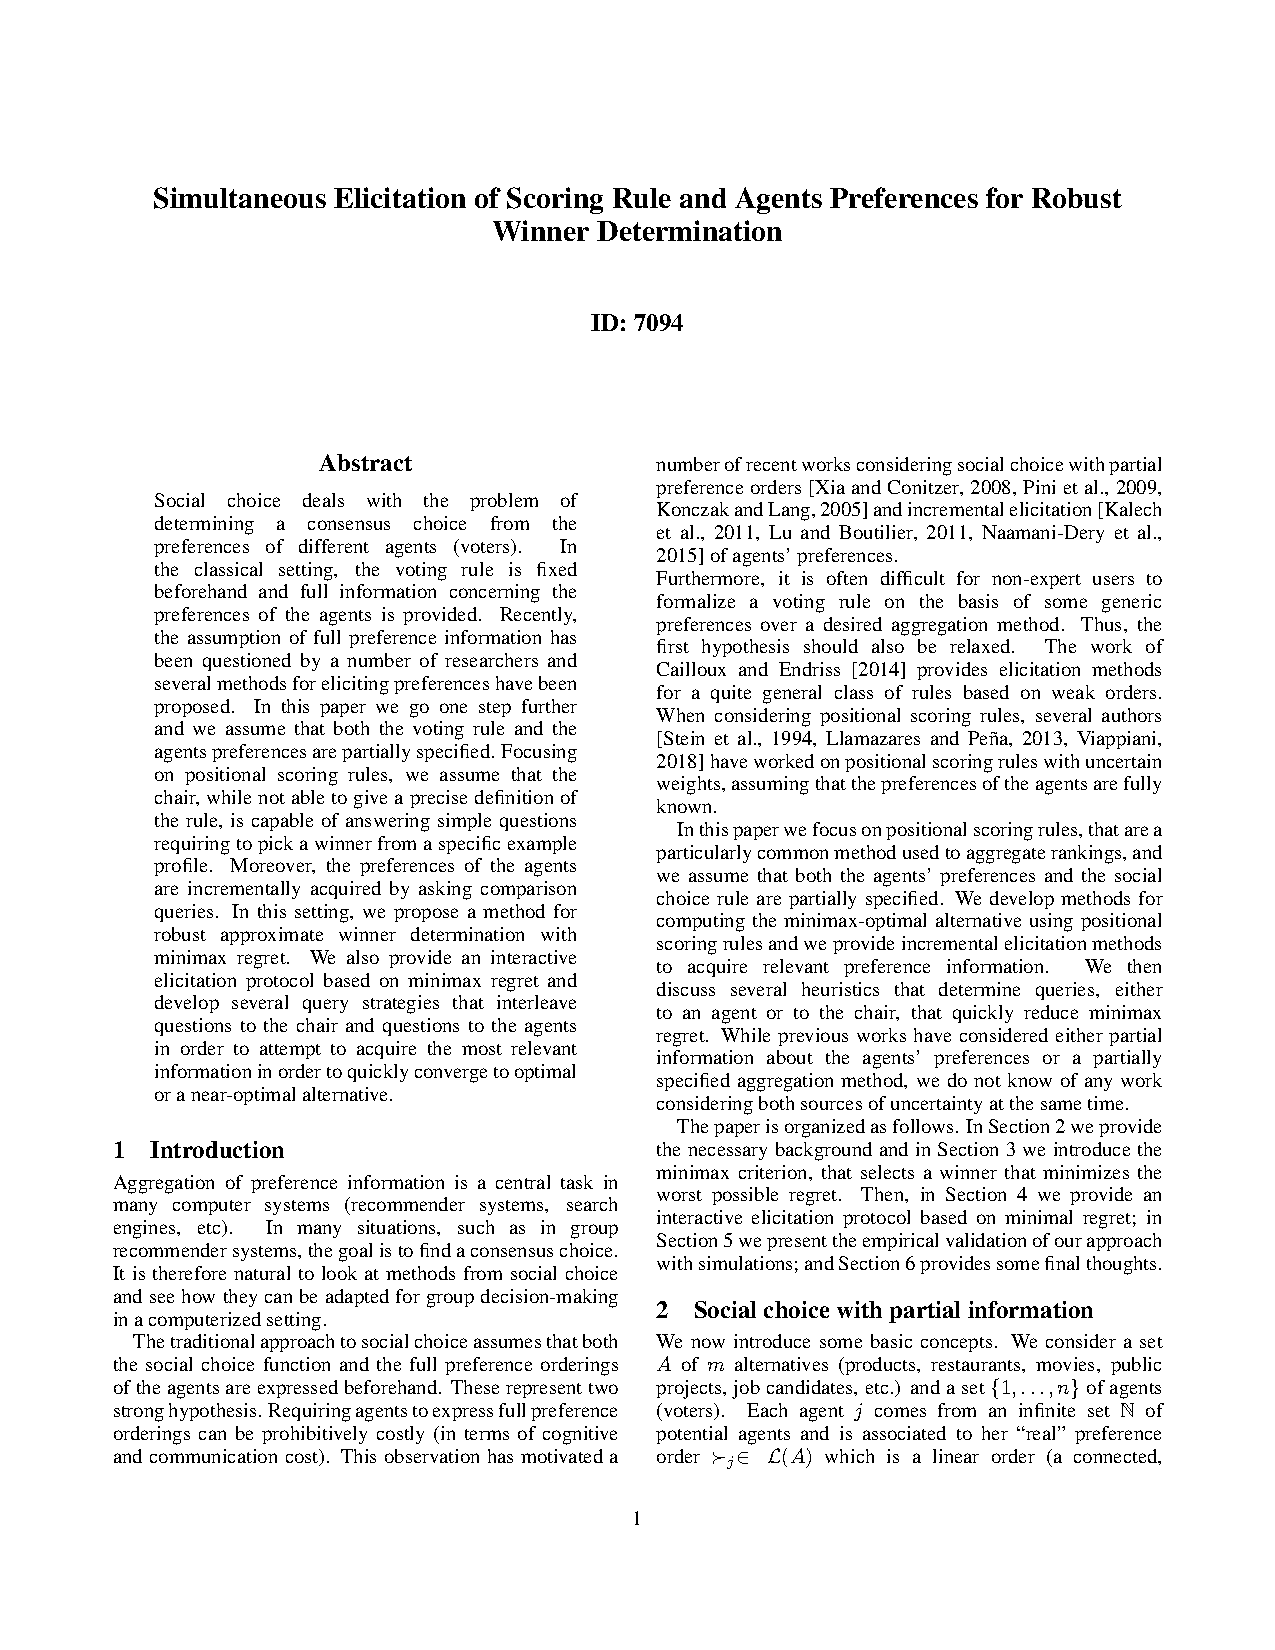
\includepdf[pages=-]{ijcai20_paper_7094.pdf}

\section{Submission to AAMAS 2021} 
\label{sec:reviews-aamas}
\subsection{Review 1}
\subsubsection*{Summary:}	The authors use the notion of minimax regret to guide the process of preference elicitation in an election (they elicit both the voters' preferences and the preferences of the chair regarding the scoring rule used). The authors show that the methodology of Lu and Boutilier for computing minimax regret still applies in their setting and present some experimental results.
\subsubsection*{Strengths:}	1) Minimax regret is a rather natural notion, which has not received much attention so far.
\subsubsection*{Weaknesses:}
1) The theoretical results are relatively simple extensions of the results of Lu and Boutilier
\newline 2) The experimental results seem quite preliminary.

\subsubsection*{Detailed comments:}	The paper is quite well written, clear, relevant for the conference. The biggest issues I have regard significance. The idea of using minimax regret to guide elicitation is very good, but is explored quite well by Lu and Boutilier. Here the authors extend this framework by eliciting the scoring rule used, but there is very little discussion as to why this really is such a good idea. I cannot easily think of a half-realistic setting where one would know that the scores need to be convex, but at the same time one would not know which ones exactly to use.

More specific comments come below:
\begin{enumerate}
\item Related work \\
As the paper is partially related to designing/choosing a scoring rule for a given setting---and as the problem of manipulation is mentioned---it might be worth to consider the following paper:

Dorothea Baumeister, Tobias Hogrebe:
Manipulative Design of Scoring Systems. AAMAS 2019: 1814-1816

Regarding partial preferences and manipulation, one may also look at the following one (although it is less related, for sure):

Dorothea Baumeister, Piotr Faliszewski, Jérôme Lang, Jörg Rothe:
Campaigns for lazy voters: truncated ballots. AAMAS 2012: 577-584


\item Concurrent elicitation of the scoring rule \\
I am not really convinced that the assumption that a scoring rule is not known makes sense. On the one hand, there is the problem of choosing the scoring rule manipulatively (but since the authors mention that the elections at hand are built into recommendation systems etc., this is not really an issue). The other problem is that I can hardly think of a scenario where the chair can answer the questions about the scoring rule, but somehow it is difficult for him to produce the full rule in a single step. So what do we gain?

\item Claims vs Propositions \\
I do not understand why the authors use "Claims" and not "Propositions".

\item I think that Claim 4 should say something along the lines: "There is a profile P', such that ... and P' can be computed effectively".

\item I can hardly imagine a person who faced with the profile P' from Claim 4 could meaningfully answer if a is better than b or the other way round. A piece of software could do it, though---but probably by precomputing the scoring rule to use (which removed the need for eliciation).

\item Proof of Claim 4: I do not understand notation (3,m) or (4,m-1) etc.

\item Empirical evaluation is very preliminary
I have a number of complaints regarding the evaluation process:
	\begin{enumerate}
		\item Why do the authors use IC only? Why not other statistical cultures? Why not some real-life data? After all, the experimental part is the main contribution of the paper and it is done in a fairly minimalistic way.
		
		\item Why do the authors look at very small elections only? 15 candidates and 30 voters seems completely inadequate for the motivations from the introduction.
		
		\item The conclusion that the number of questions required to reach low regret cannot be made based on Table 3. There is simply far too little data to have any sort of confidence in claims like this.	
	\end{enumerate}

\end{enumerate}

All in all, I think it is certainly a nice enough paper to be accepted as short, but is below the bar for the full acceptance.

\subsubsection*{Questions for rebuttal:}
Q1: Why did you only look at IC elections?
\newline Q2: How to use your approach in large elections? Hundreds of candidates, thousands of voters? After all, showing a strategy that can deal with large elections would meaningfully extend the work of Lu and Boutilier?
\newline Q3: Can you provide a realistic example where elicitation of the scoring rule is useful?
\subsubsection*{Score:}	
4: (poor (good attempt but too many concerns, so probably should be rejected))

\subsubsection*{Comments added after rebuttal:}
I found the example provided in the response to be convincing.

I still think that testing the heuristics on IC only is insufficient. Even if it is the hardest case, I would also like to see how the algorithm peforms in the easier ones. Can it exploit the structure when the structure is present? One cannot evaluate such issues by looking at IC alone.

\subsection{Review 2}
\subsubsection*{Summary:}
The paper studies a voting problem wherein neither the voting rule nor the voters' preferences are specified in advance. Rather, an elicitation procedure is used to determine the election winner by asking the voters questions about their preferences and asking the chair questions about the voting rule.

Specifically, the preferences of the voters are assumed to be given by a fixed set of linear orders that are unknown to the elicitation platform. In addition, the voting rule is assumed to belong to the class of positional scoring rules with monotone weights with diminishing differences. The elicitation procedure comprises of the chair specifying the winning candidates on example profiles, and the voters responding to a series of pairwise comparisons.

At each step, the minimax regret criterion (Lu and Boutilier, IJCAI'11) is used to determine the next query, and this procedure is continued until convergence (e.g., either the regret drops below a certain threshold or a certain number of questions have been asked). The regret of an alternative, informally speaking, is the "loss" incurred for picking that alternative instead of an "optimal" one under adversarial choice of completion of the partial preferences elicited so far as well as the worst-case choice of positional weights.

The main contributions of the submission are:
1. Proposing a framework for simultaneously eliciting voters' preferences and information about the voting rule based on the minimax regret criterion.
2. Experimental comparison of a number of elicitation heuristics in terms of the number of questions asked or the regret value.

The empirical observations suggest that a modest number of questions (to the voters as well as the chair) are sufficient in arriving at a reasonable choice, and that the regret drops super-linearly as a function of the number of questions asked over the course of elicitation.
\subsubsection*{Strengths:}	The idea of modeling simultaneous uncertainty in the voting rule as well as the voters' preferences is quite interesting. It is also useful to know that the minimax regret framework of Lu and Boutilier (IJCAI'11), previously studied in the setting of a known voting rule, can be extended to the aforementioned more general problem.
\subsubsection*{Weaknesses:}	The lack of theoretical guarantees for the proposed elicitation strategy, as well as missing reasoning behind several of the experimental observations, makes this a weak paper in my opinion.

\subsubsection*{Detailed comments:}
I like the high-level question asked by the paper, namely whether it is possible to simultaneously elicit the information about the voting rule and the voters' preferences. However, the significance of the contribution is less clear. The results, which largely comprise of experiments, are at the level of proposing a heuristic that seems to work well in simulations but lacks formal theoretical guarantees.

I believe the paper will be much stronger if the authors could provide theoretical convergence guarantees for the proposed heuristics. Additionally, in the "Empirical Evaluation" section, instead of simply describing the observations, it would be useful to also formally state the hypotheses used in each experiment, and explain how the experiments support or refute those hypotheses. For example, you could describe whether (and why) one might expect "Pessimistic" strategy to work better than the "Elitist" strategy, and then discuss to what extent did the simulations confirm that hypothesis.

Some minor comments are below.
\begin{enumerate}
\item Page 1
\begin{itemize}
	\item In several places you use the phrase "permits to" when it might be clearer to say "allows for".
\end{itemize}

\item Page 2
\begin{itemize}
	\item "that showed that"-->who showed that.
\end{itemize}

\item Page 3 
\begin{itemize}
	\item "there are no necessary winner"-->there is no necessary winner.
\end{itemize}

\item Page 4 
\begin{itemize}
	\item "less good than or equal to"-->You could rather say "weakly worse".
	\item Using $\succeq^p_j(x)$ to denote the set of alternatives weakly worse than x can be confusing. Please consider using a different notation such as $A^(\succeq^p_j,x)$.
\end{itemize}

\item Page 5
\begin{itemize}
	\item Claim 4 is written in the form of a definition, and it is not clear what is actually being claimed here. Maybe you could say that "there exists a profile P' satisfying such and such properties".
	\item "each of the p+q agent"-->each of the p+q agents
	\item "worst than"-->worse than
\end{itemize}

\item Page 6 
\begin{itemize}
	\item "on order to"-->in order to
	\item "an important weight"-->a large weight
	\item "For generating the weights we first draw $m - 1$ numbers uniformly at random"-->What is the range from which you make the draws?
\end{itemize}

\item Page 7 
\begin{itemize}
	\item "In-dept evaluation"-->In-depth evaluation
	\item Figure 1, X axis label should say "Number of questions"
	\item "to be ran"-->to be run
	\item "We see that the number of questions required to reach a low regret level grows approximately linearly with the number of agents"-->Can you provide a formal regression analysis to support this claim?
\end{itemize}

\item Page 8 
\begin{itemize}
	\item "allow to quickly"-->allows to quickly
	\item "worst regret"-->worst-case regret
	\item "that allows to reproduce our experiments, and more"-->It would be useful to mention the other benefits explicitly.
	\item "halving the number of questions will only reduce the gain in regret by less than half"-->Might be clearer to say "halving the number of questions reduces the regret by more than 50$\%$".
\end{itemize}

\end{enumerate}
\subsubsection*{Questions for rebuttal:}	1. On Page 1, you write that "The quality of the recommendation increases faster than linearly with the number of questions, after an initial phase with almost no increase in quality, before slowing down and converging to an optimal recommendation." What is the reasoning behind this trend?
\newline 2. How did you decide the range of the parameter $\lambda$ to be [1,n]?
\subsubsection*{Score:}	
4: (poor (good attempt but too many concerns, so probably should be rejected))

\subsubsection*{Comments added after rebuttal:}
Thanks to the authors for responding to the questions raised in my review. My concern about the significance of the paper remains. In the absence of any formal theoretical guarantees about the performance of the elicitation heuristic, the paper will likely be of limited interest. The authors note that obtaining such guarantees could be difficult. Nevertheless, the paper could certainly benefit from a revised experimental analysis that clearly formulates the hypotheses to be tested and how the experiments support or refute those hypotheses.

\subsection{Review 3}
\subsubsection*{Summary:}
This paper considers elicitation in the context of scoring rules when both the preferences of the voters and the weights defining the rule might be missing. The authors model the problem via regret minimization and propose several types of queries and querying strategies. The paper also presents an interesting experimental study which supports the presented approach.
\subsubsection*{Strengths:}	The problem addressed is interesting and has potential for practical applicability.
Addressing missing information in both voters and the chair’s preferences is novel. The experimental section is a good starting point.
\subsubsection*{Weaknesses:}	The discussion on the motivation behind considering uncertainty on the scoring rule’s weights is not very convincing. They claim the chair might not be able to formalize the rule…
Another point that is not clear is when, in practice a system like this would be deployed.
The application of regret minimization is somewhat incremental w.r.t. the literature.

\subsubsection*{Detailed comments:}	reference elicitation in the context of voting is certainly a relevant topic for AAMAS.
The setting considered here is not per se novel, as elicitation of voters’ and the chair’s preferences have been considered before. The originality lies in considering them both at the same time.
While this is original, the motivation of when such a setting may occur in practice is not clear. In particular, I wonder about the timing. It is assumed that voters and candidates are known, information about the voters preferences is available and yet the voting rule has not yet been decided and the elicitation process is going on at the same time. It seams unlikely to me.
As I mentioned, I am also not very convinced about a chair not knowing which rule he wants/or is using while voters are expressing preferences. A much stronger argument would be that of a third party discovering information about a voter’s preferences and the rule by being able to observe results or to tap in and acquire some information. Obviously that would mean having much less control over what information is acquired than assumed here…it might be similar to random strategy studied in the experimental section.

The content is technically not overly sophisticated, so I have no doubt about its soundness.
The presentation flows well and all parts are clearly written. The description of the experimental results is also sufficiently detailed to enable reproducibility.

A minor complaint is that Figures 1 and 2 are blurred.
\subsubsection*{Questions for rebuttal:}
1) Could testing mixed strategies yield better results than the pure ones?
\subsubsection*{Score:}	
7: (good (probably should be accepted))

\subsection{Metareview}
The main reason for the reject recommendation is the missing novelty in this paper. It basically is a reimplementation of the ideas from Lu and Boutilier. Furthermore, in the experimental section, clear hypotheses are missing and the reasons for limiting the analysis to IC are not convincing.

\subsection{Our rebuttal}
Our proposal is methodologically innovative: it addresses in a new way the difficult problem of eliciting preferences about voting rules. It opens up a novel path to gather and exploit preferential information about voting rules, in parallel with more classical preferential information about the alternatives under scrutiny. As a result, multiple challenging research questions open up, several of which are raised by the reviewers. We warmly thank them for these observations.

As reviewer 1 points out, one could simply ask for direct information about the parameters of the rules, such as the weight vector. But it is unclear whether the answers to such questions would be meaningful. For example, in many cases, the chair (supposed to be human) may not know whether the largest weight should be twice, or three times, the weight associated with the second rank.

We ask the chair which alternative should win given a concrete profile. Such questions have precise semantics whose understanding is shared by the chair. This way of asking questions is sufficiently natural that it has been used in experimental settings investigating the feeling of justice of individuals (Does majoritarian approval matter in selecting a social choice rule? An exploratory panel study, Ebru Giritligil and Sertel, Social Choice and Welfare 25(1):43-73, 2005). To the best of our knowledge, the use of such questions to systematically guide an elicitation process is novel. We will highlight this aspect in the paper.

Our approach is analogous to that of decision theorists with preference elicitation: a large stream of research considers more meaningful to ask direct choice questions ("please choose either a or b") than to question the decision maker about the shape of its utility function. The former are considered "observable": acts of choice are translated to preference statements.

Concerning the hypothesis of convexity raised by reviewer 1, we need to assume that we look for a function inside a specific class of functions (here, the scoring rules with convex weights) because the class of all possible functions is too large. This allows for mixing an axiomatic basis with more precise "observable" questions; again, as it is usually done in decision theory (which often assumes the Subjective Expected Utility axioms). The use of convex weights is a natural and common assumption: losing ranks at the top of the ranking is more damaging than losing ranks at the bottom.

A concrete application of our work might be a committee that is about to hire a new employee, whose performances are evaluated by several experts. The members of the committee may not have a voting rule in mind at the start of the process, and might not wish to agree on a specific voting rule, but they might be willing to answer enough questions about selecting winners out of specific profiles to determine their employee of choice.

Regarding the experimental concerns addressed by reviewer 1, our strategies and setting are meant to tackle small scale social choice situations such as just exemplified. Our questioning method, in particular, does not scale to hundreds of candidates because the chair must be assumed to have limited cognitive capacity.

IC is a quite challenging situation: as can be expected intuitively (and shown experimentally by Lu and Boutilier in their setting), the number of questions to be asked decrease with less varied profiles. We want to focus on the most critical setting, as there is a wide variety of possible situations to test in such experiments.

The reviewers are right to point out that our comments about Table 3 were overconfident, this will be corrected.

Reviewer 1 Question6 : We should have written “given to c the ranks 3 and m” instead of (3, m) in the proof of Claim 4.

Reviewer 2 Question2: The $\lambda$-range is initialized to [1,n] because $\lambda \geq1$ by convexity and we assume $\lambda \leq n$ wlog: for $\lambda \geq n$, the rule coincides with Plurality.

Regarding the guarantees concerns raised by reviewer 2: The general lack of theoretical guarantees with respect to the number of questions in the literature adopting minimax regret approaches suggest that obtaining such results is very difficult, if possible. However, our approach guarantees to return the true winners when the elicitation is completed. Note that the process can be terminated early, and offers a guaranteed bound on the regret at any time.

Reviewer 2 Question1: At the start of the elicitation, the space of uncertainty is so large that the adversary can attain the maximum possible value of regret; multiple answers are needed to constrain her enough for the MMR to start decreasing. When approaching optimality, the pace of MMR reduction decreases.

Reviewer 3 Question1: We did not investigate a systematic way of mixing strategies but we manually mixed different ideas in order to obtain the strategies we presented. For example Two phase and Extended Pessimistic reuse ideas present in the Pessimistic strategy.

\section{Rejected paper AAMAS 2021}
You will find here below the version of this article that was submitted to AAMAS 2021.
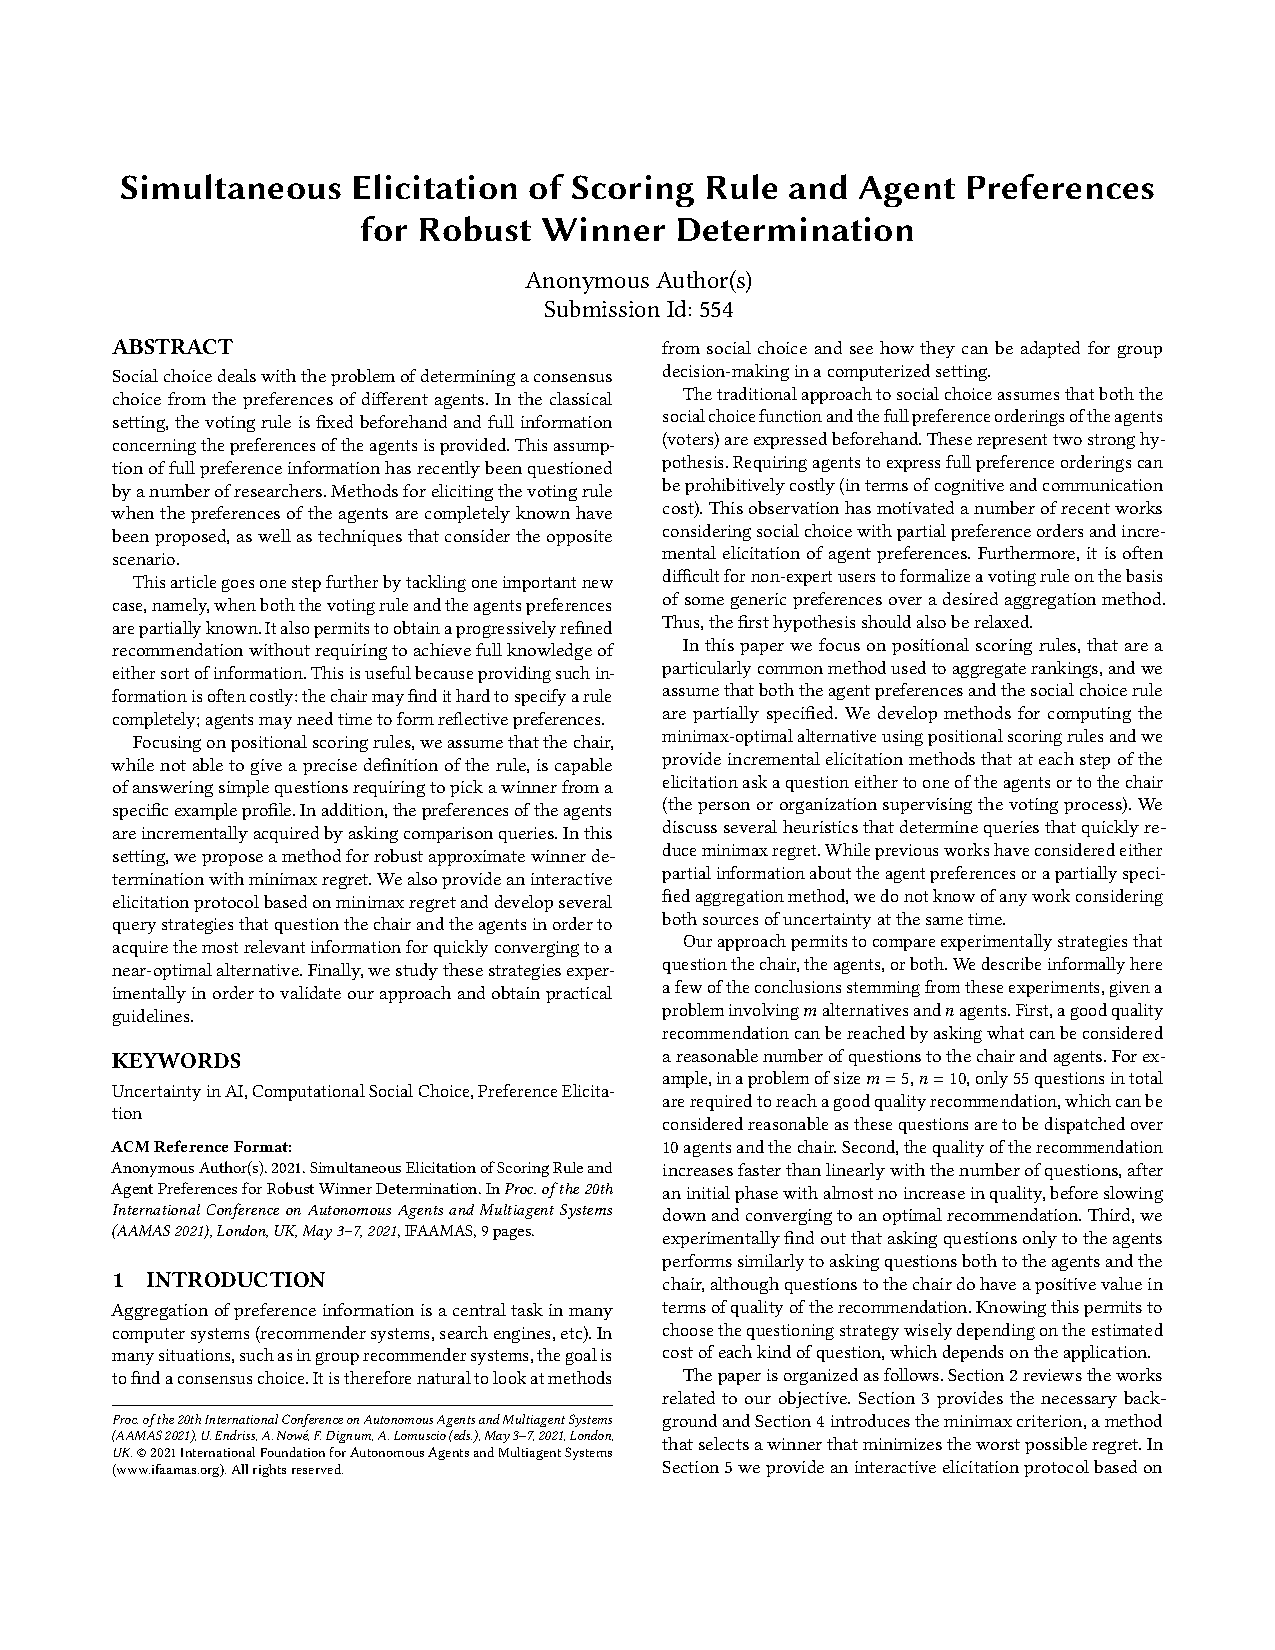
\includepdf[pages=-]{aamas21_paper_554.pdf}
\end{document}
